\section{Technique and implementation}
%% \label{sec:approach}

\begin{figure*}
  \centering
  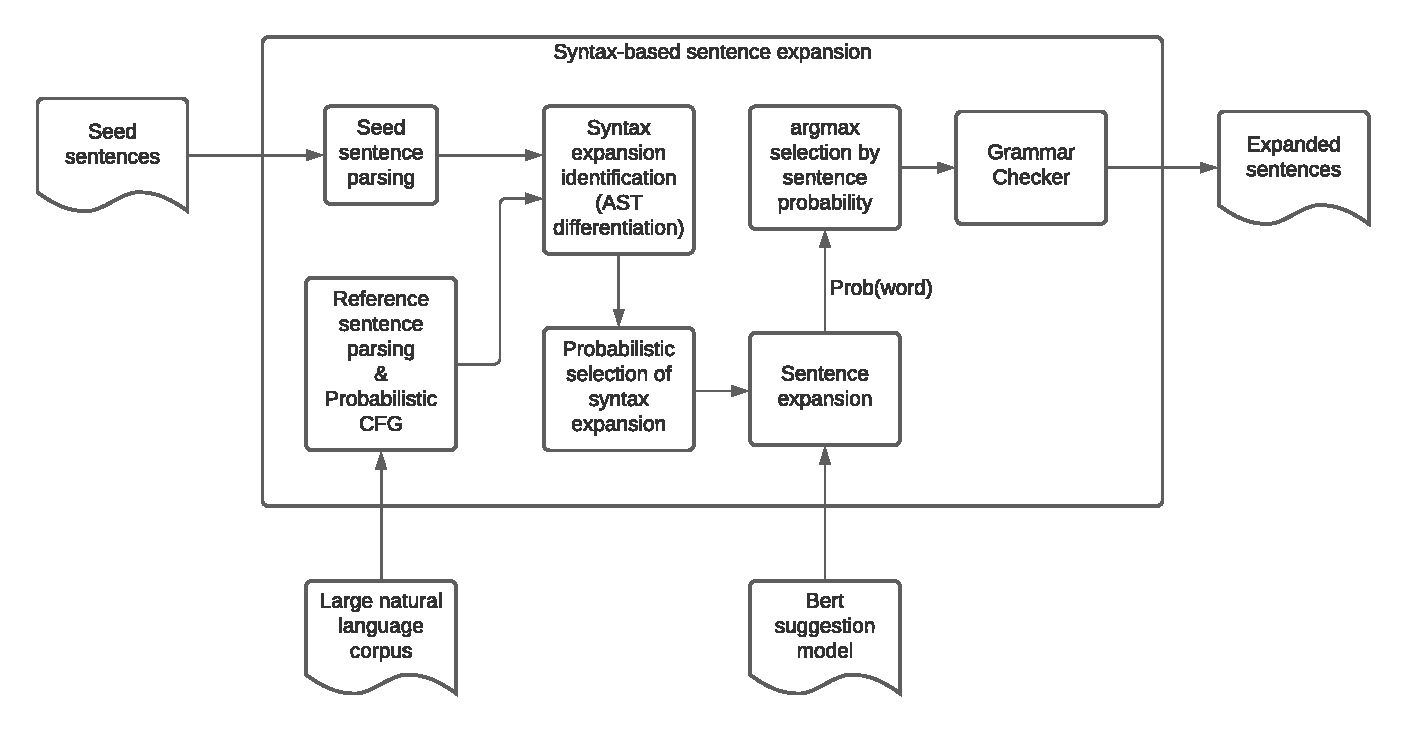
\includegraphics[scale=0.5]{figs/overall.pdf}
  \vspace{-5pt}
  \caption{\OverallModelFigCaption}
  \vspace{-10pt}
\end{figure*}

\Model generates input sentences with the following phases illustrated
in \ref{fig:OverallModel}: 1. search phase searches seed sentences according to
its requirement of \lc, 2. seed parsing phase parses the found seed
sentences and extract their \cfg, 3. reference phase collects large
corpus, 4. syntax expansion identification, and 5.sentence expansion
and generation. In this section, we provide more details on each phase.

\subsection{Search phase}
The search phase in \Model searches and samples subset of sentences in the
dataset that meets the requirement extracted from each linguistic
capability. Each linguistic capability represents performance of \nlp
task on specific input domain

requires certain format of sentences

